\documentclass[12pt]{article}

\usepackage[utf8]{inputenc}
\usepackage{titling}
\usepackage{floatrow}
\usepackage{graphicx}
\usepackage[english]{babel}
\usepackage{amsmath}
\usepackage[ruled, lined, linesnumbered, commentsnumbered, longend]{algorithm2e}
\usepackage{hyperref}
\usepackage{lastpage}
\usepackage{enumitem}
\usepackage{multicol}
\usepackage{multirow}
\usepackage{fancyhdr}
\usepackage{xcolor}
\usepackage{listings}
\usepackage[a4 paper, includefoot, hmargin = 1 in, top = 1 in, bottom = 0.75 in]{geometry}

\RestyleAlgo{ruled}
\SetKwComment{Comment}{/* }{ */}
\setlength{\tabcolsep}{25pt}
\renewcommand{\arraystretch}{1.5}
\setlength{\arrayrulewidth}{0.5mm}
\setlength{\headheight}{14.5pt}
\bibliographystyle{IEEEtran}
\hypersetup{colorlinks=true,urlcolor=blue,linkcolor=black}
\renewcommand\maketitlehooka{\null\mbox{}\vfill}
\renewcommand\maketitlehookd{\vfill\null}
\renewcommand{\footrulewidth}{0.4pt}

\lstset{
    numbers = left,
    frame = lines ,
    breaklines = true,
    keywordstyle = \color{blue}\bfseries,
    showstringspaces = false ,
    numberstyle = \tiny\color{gray},
    commentstyle = \color{green!30!black},
    stringstyle = \color{violet}
}

\renewcommand{\lstlistingname}{\bfseries \large Listing}
\makeatletter
\def\fnum@lstlisting{%
  \lstlistingname
  \ifx\lst@@caption\@empty\else~\thelstlisting\fi
  }%
\makeatother

\title{\textbf{\huge Software Systems Lab: OutLab \LaTeX}}
\date{\LARGE \today}
\author{\Large Name: Atishay Jain \\ Roll no: 210050026}

\pagestyle{fancy}
\renewcommand{\headrulewidth}{1pt}
\fancyfoot[C]{\thepage\ of \pageref{LastPage}}

\begin{document}

\begin{titlingpage}
    \maketitle    
\end{titlingpage}

\tableofcontents

\newpage

\section{Introduction}
\vspace{1 em}
This report consists of work done by me under \textbf{CS 251} course. This is a \textit{Software Systems Lab} course that teaches many different kinds of programming utilities that are used by programmers quite often. This course is all about to help the students in the later courses. 

\subsection{Course Content}
\begin{table}[H]
    \centering
    \begin{tabular}{ |c|c| }
         \hline
         \textbf{S.N.} & \textbf{Topic} \\
         \hline
         1 & HTML/CSS and Java Script \\
         \hline
         2 & Bash Basics + Git + Markdown \\
         \hline
         3 & SED and AWK \\
         \hline
         4 & \LaTeX \hspace{0.2 ex} Basic + Advanced \\
         \hline
         5 & Python Basics and Advanced \\
         \hline
         6 & Web-scraping / DB / Networking \\
         \hline
         7 & Java Basics \\
         \hline
         8 & Make/Cmake \\
         \hline
         9 & Doxygen and Sphinx \\
         \hline
    \end{tabular}
    \caption{Topics taught under CS 251 course}
    \label{tab:my_label}
\end{table}
Although there are many topics, but this report will be mainly based on my works and learning about \textbf{Linux}, \textbf{Bash}, \textbf{Sed} and \textbf{awk}.

\subsection{Goal}
\begin{itemize}
    \item Presenting your work using HTML, CSS, Drawing Software, \LaTeX, gnuplot
    \item Code Warrior via reading \& writing code, profiling, Debugging, learning about Editors, IDE, Compilation, Version Control, Bash, Awk etc.
    \item Learning about Open Source Operating System - \textbf{Linux}
    \item Prepare students with the vocabulary of CS tools such that later concepts can be easily explored
\end{itemize}

\newpage

\section{Linux - An Open Source Operating System}
\textbf{Linux}\cite{Linux:1} was developed and publicly released by ``Linus Torvalds" in September 1991. Linux is a free and open-source operating system, unlike either Windows OS or macOS. Various Linux Distros are available and are free to use. Typically the Linux OS is employed for cloud and server software. Some popular Linux distros are \textit{Ubuntu, Debian, Fedora} etc. Because Linux is free and open-source, it allows end-users to freely alter, utilize, distribute, and publish software code. \\

\subsection{Why Linux?}
Programmers and Developers mostly use Linux\cite{whyLinux:3} for Coding and learning Computer Science. Linux\cite{whyLinux:2} is preferred over other OS because -
\begin{enumerate}
    \item Linux tends to be highly reliable and secure system than any other OS -
    \begin{enumerate}[label=(\roman*)]
        \item As it is open source, huge number of programmers and developers are fixing the issues and reviewing the code, and hence it has lesser security flaws.
        \item You don't need antivirus to protect from malware or viruses because of its security.
        \item Linux has more privacy. Windows collects some user data but in Linux, you can always look into its source code and literally see everything transmitting from your system.
    \end{enumerate}
    \item It is free to use, Open Source and Developer friendly
    \begin{enumerate}[label=(\roman*)]
        \item It is freely available, saves money on licenses and software.
        \item It has powerful and helpful software managers like apt, rpm , dpkg, synaptic etc that make installation process easier.
        \item A lot of handy useful and Powerful programming tools comes pre-installed with Linux like grep, wget, cron etc that makes it developer friendly.
    \end{enumerate}
    \item Task Automation and Command Line Interface
    \begin{enumerate}[label=(\roman*)]
        \item Linux offers several shells such as \textbf{Bash}, SH, Korn, ZSH, Fish through which users can automate thier tasks easily.
        \item The shell can not perform its magic until the end-user types some commands in the command-line interface (CLI) through the Linux Terminal.
        \item Linux terminal is kind of the \textit{heart of Linux}. It is very efficient and faster.
    \end{enumerate}
\end{enumerate}

\subsection{Some other Features in Linux}
Linux has many different features unique to it. Such as a powerful editor known as \textbf{Vim}, task automating shells such as \textbf{Bash}, text editing streams like \textbf{SED} and \textbf{AWK}, version control from Command line using \textbf{Git} and many more. These features come very handy in use for any programmer and thus programmers should know about these and be well-versed in thier usage. Let's see more about some of them.

\newpage

\section{Bash Scripting}
\vspace{1 em}
The \textbf{Linux Bash}\cite{Bash:4}, also known as `Bourne-again Shell' is a command language interpreter for the Linux based system. It is a replacement of Bourne shell (sh). It was developed under the GNU Project and written by \underline{Brian Fox}. The Linux/Unix shell allows us to interact with the Linux system through the commands. It let us invoke an executable file to create a running process. \\
The Bash is a command language interpreter as well as a programming language. It supports variables, functions, and flow control, like other programming languages. It can also read and execute the commands from a file, which is called a \textbf{Shell Script}\cite{LinuxBash:5}. Some key features of Bash are Shell syntax, Shell commands, Shell functions, Shell parameters, Redirections, Command executions and Shell scripts.

\subsection{What is Shell \& Scripting?}
\vspace{1 em}
    \fbox
    {
    \begin{minipage}{0.4\textwidth}
        \begin{center}
            \large{\textbf{Shell}}
        \end{center}
        If we are a new Linux user, and we open the terminal, it is assumed that we are well confused as to what to do with it. Here the Shell comes in the role.
        The terminal contains the shell; it allows us to execute the commands to interact with the system. We can perform various operations such as store and retrieve data, process information, and various other simple as well as complex tasks.
    \end{minipage}
    }
    \hfill
    \fbox
    {
    \begin{minipage}{0.4\textwidth}
        \begin{center}
            \large{\textbf{Scripting}}
        \end{center}
         Suppose we want to run a series of commands many times to perform a task. Instead of doing the same process many times, Linux supports a feature called scripting that allows to execute more than one task at once. So, it is good to define a script rather than performing repetitive tasks. Script is a file that consists of commands that we want to run. To define a script, we create a file with a .sh extension
    \end{minipage}
    }
\vspace{1 em}

\subsection{More Features of Bash}
\vspace{1 em}
Well, not only basic commands, we can do many more things using a bash script. Just think about it, Bash can perform those tasks also that a programming language like C++ does it can also execute the commands that we use to write on terminal using \textbf{CLI}. A simple example can be that Suppose you are working on a C++ code that involves linking and compilation of several object modules and command line arguements. Now, instead of comipiling all those cpp files to make object modules and then linking them, you can just make a Bash script that will do it for you in a single run. \\
Also, many other Linux features like SED, AWK, Git, etc can be used within a Bash Script when you are using them for a more complex task.

\section{Task Automation using Bash}
\vspace{0.5 em}
\subsection{Background}
\vspace{1 em}
Zomato food delivery needs a persistent storage which can store the information of their customers along with their order details.They need to store Customer's first name and Order ID.Along with this information they also need to keep track of time at which this data is stored in persistent storage.You need to create such storage using files. \\
You need to make a script that will can perform following tasks - 
\begin{enumerate}
    \item  \textbf{storeInfo}: Create an entry for $<$CustomerName, Order ID$>$ pair in storage along with the time and date at which the order was placed.
    \item \textbf{displayInfo}: Display information of Customer Name and Order ID on terminal.
    \item \textbf{getOrderID}: Display the Order ID associated with a given Customer Name
\end{enumerate}

\subsection{Solution with Bash Code}
If we would be using any other simple Document for storing this data, it would have been so problematic to keep track the date and time whenever we insert a new entry into our storage and also for finding a particular entry in the storage. But using a Bash Script, we can automate this task easily. \vspace{1 em} \\
\textbf{\large Algorithm} \vspace{1 ex} \\
The first two functions implementation is quite simple and normal, but the last one is a bit tricky. So, let's have a look on the algorithm that can be used for getOrderID funcrion followed by the complete Bash Script code file named as \texttt{script.sh} - 
\begin{algorithm}[hbt!]
\SetKwInOut{KwIn}{Input}
\SetKwInOut{KwOut}{Output}
\KwIn{Name of the text file (fileName) and Name of customer (name) as command line arguement}
\KwOut{Order IDs and details of order by given customer}
\SetAlgoLined
\SetKw{Print}{print}
\SetKwProg{Fn}{Function}{}{end Function} 
\Fn{getOrderID() : }{
    $N \gets$ numberofOccurence(name,fileName) \Comment*[r]{by using grep $|$ wc}
    $x \gets$ listofOccurence(name,fileName) \Comment*[r]{by using grep command}
    $j \gets 0$\;
    \For{$i$ \textbf{in} $x$}{ 
        \If{$j$ mod $2 \neq 0$}{ 
            \Print i \Comment*[r]{only IDs of given name will be printed}
        }
        $j \gets j + 1$ \Comment*[r]{because name \& ID are stored alternatively}
    }
    \Print N\;
}
\caption{Algorithm for getOrderID function}
\end{algorithm} \\
Following is the implementation of the solution using Bash - 
\begin{lstlisting}[language=bash,caption=Bash Script]
#!/bin/bash
now="$(date+'%d/%m/%Y')"       #'date' returns today's Date
time=$(date+"%T")
name=$2
underScore="_"
Name="$name$underScore"
id=$3
function storeInfo(){          #Store info of an Order entry 
    echo ${name}_${now}-${time} ${id} >> store.txt
}
function displayInfo(){        #Display all Order entries info
    echo Name OrderID
    cat store.txt
}
function getOrderID(){         #Get Order info of a given Name
    echo "OrderID's found are:"
    number=$(tr ' ' '\n' < store.txt | grep $Name | wc -l)
    found=$(grep $Name store.txt)
    j=0
    for i in $found
    do
        if [ $(expr $j % 2) != "0" ]; then
            echo $i
        fi 
        j=$(($j+1))
    done
    echo "$name" ordered "$number" times
}
"$@"
\end{lstlisting}
We can run the above script for performing the required tasks -
\begin{enumerate}
    \item \textbf{storeInfo}
    \begin{itemize}
        \item For storing an Order ID pair, let's say ``Atishay" ``2552", we can run the above script as - \texttt{./script.sh storeInfo Atishay 2552}
    \begin{figure}[H]
        \centering
            \begin{floatrow}
            \ffigbox[0.8\textwidth]{\caption{\texttt{cat} command is used here to display content of a file}}{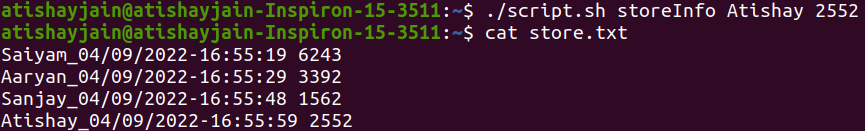
\includegraphics[width=0.8\textwidth]{storeInfo.png}}
            \end{floatrow}
    \end{figure}
        \item The storeInfo function 
        \begin{itemize}
            \item echoes the string of name, OrderID and other data using \texttt{echo} command 
            \item and redirects it to a storage file \texttt{store.txt} using \texttt{>>} operator
        \end{itemize}
    \end{itemize}
    \item \textbf{displayInfo}
    \begin{itemize}
        \item For displaying all the Order ID's stored in our storage, run the script as - \texttt{./script.sh displayInfo}
        \item The displayInfo function
        \begin{itemize}
            \item echoes the string ``Name OrderID"
            \item uses \texttt{cat} command to display store.txt
        \end{itemize}
        \begin{figure}[H]
        \centering
            \begin{floatrow}
            \ffigbox[0.8\textwidth]{\caption{combination of above two statements results in such a display}}{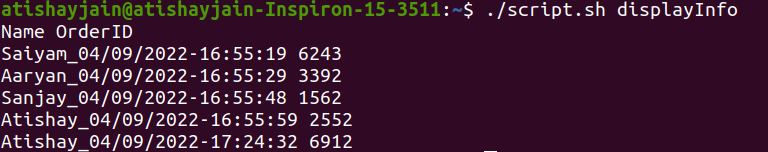
\includegraphics[width=0.8\textwidth]{displayInfo.png}}
            \end{floatrow}
        \end{figure}
    \end{itemize}
    \item \textbf{getOrderID}
    \begin{itemize}
        \item To get the Order ID's corresponding to a given name, let's say ``Atishay", run the script as \texttt{./script.sh getOrderID Atishay}
        \begin{figure}[H]
        \centering
            \begin{floatrow}
            \ffigbox[0.8\textwidth]{\caption{It displays all the Order IDs and number of orders by Atishay}}{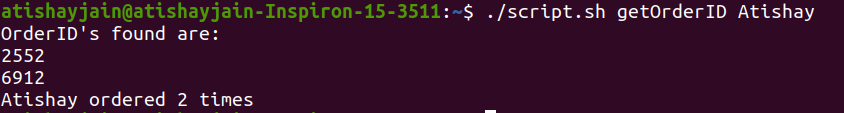
\includegraphics[width=0.8\textwidth]{getOrderID.png}}
            \end{floatrow}
        \end{figure}
        \item The getOrderID function uses
        \begin{itemize}
            \item \texttt{echo} command at appropriate places to print some text
            \item \texttt{grep} command which is used to search for a string in a file
            \item \texttt{wc} command which is used for finding word count, line count, character count etc
            \item \texttt{tr}\cite{tr:6} command which is used to translate/delete characters from input and writes the result to output
            \item $|$ symbol, that is used for piping. Piping means using output of previous command as input for next command
            \item and a for loop using which it finds and prints the order ID and number of orders after looping through the whole storage file
        \end{itemize}
    \end{itemize}
\end{enumerate}
More information about various such Linux Commands and Bash can be found \href{https://www.javatpoint.com/linux-commands}{here}.

\newpage

\section{Sed}
\textbf{Sed}\cite{Sed:7} is the ultimate \textcolor{red}{\textbf{S}}tream \textcolor{red}{\textbf{ed}}itor, which can be used to perform lots of functions on file like searching, find and replace, insertion or deletion. Though most common use of SED command in UNIX\cite{Sed:8} is for substitution or for find and replace. By using SED you can edit files even without opening them, which is much quicker way to find and replace something in file, than first opening that file in VI Editor and then changing it.
\begin{itemize}
    \item SED is a powerful text stream editor. Can do insertion, deletion, search and replace(substitution).
    \item SED command in unix supports regular expression (\textit{Regex}) which allows it perform complex pattern matching.
\end{itemize}

\subsection{Background}
To understand the power of Sed, let's analyze a situation. Suppose we have a list of emails and we want to check the emails that are valid in this list. Manual checking for a large number of such emails will be very complicated and will take a lot of time and inefficiency. Sed can do this very fast and efficiently.

\subsection{Work Done}
We will use Sed command inside a Bash Script for validating email addresses. The code is following -
\begin{lstlisting}[language=bash,caption=Using Sed inside a Bash Script]
#!/bin/bash

# Run the script as : ./q1.sh <filename>
# where <filename> is the name of file containing
# the list of many email addresses

sed -n -E -e '/^[a-z0-9A-Z_\!%\+\#\&\$=\?\^~`\/\-]+[\.]?[a-z0-9A-Z_\!%\+\#\&\$=\?\^~`\/\-]+[@]{1}[a-z]+[\.]{1}[a-z]+$/p' -e '/^[a-z0-9A-Z_\!%\+\#\&\$=\?\^~`\/\-]+[\.]?[a-z0-9A-Z_\!%\+\#\&\$=\?\^~`\/\-]+[@]{1}[a-z]+[\.]{1}[a-z]+[\.]{1}[a-z]+$/p' < $1 > valid.txt

# The validated correct email addresses will be printed
# inside a new file named ``valid.txt"
\end{lstlisting}
\vspace{1 em}
The above code uses Regular Expressions and checks each email address. If the expression matches, then it prints those valid emails into a new file. \texttt{-E} tag activates the Regex expressions. \texttt{/p} at the end is used for printing in Sed, \texttt{-n} and \texttt{-e} tags are used for printing only when expression matches and using multiple commands in sed respectively.

\newpage

\section{Awk}
\vspace{1.5 em}
\noindent\begin{minipage}{0.5\textwidth}

\includegraphics[width=\linewidth]{awk.jpg}
\cite{fig:Awk}
\end{minipage}
\hfill
\begin{minipage}{0.5\textwidth}\raggedleft
\textbf{Awk}\cite{Awk:9} is a scripting language, abbreviated from the name of its developers – \textbf{\textcolor{violet}{A}}ho, \textbf{\textcolor{violet}{W}}einberger, and \textbf{\textcolor{violet}{K}}ernighan. It is used for manipulating data and generating reports. The awk command programming language requires no compiling and allows the user to use variables, numeric functions, string functions, and logical operators. \vspace{1 em}
\end{minipage}
 Awk is a utility that enables a programmer to write tiny but effective programs in the form of statements that define text patterns that are to be searched for in each line of a document and the action that is to be taken when a match is found within a line. Awk is mostly used for pattern scanning and processing.
 Awk searches one or more files to see if they contain lines that matches with the specified patterns and then perform the associated actions. 

\subsection{What can awk do?}
\begin{table}[H]
    \centering
    \begin{tabular}{|c|c|}
         \hline
         \multirow{4}{*}{Awk Operations\cite{Awk:10}} & Scans a file line by line \\ \cline{2-2}
         &  Splits each input line into fields \\ \cline{2-2}
         & Compares input line/fields to pattern \\ \cline{2-2}
         & Performs action(s) on matched lines \\ 
         \hline
         \multirow{3}{*}{Programming Constructs} & Format output lines \\ \cline{2-2}
         & Arithmetic and string operations \\ \cline{2-2}
         & Conditionals and loops \\ \cline{2-2}
         \hline
         \multirow{2}{*}{Useful For} & Transform data files  \\ \cline{2-2}
         & Produce formatted reports \\ 
         \hline
    \end{tabular}
    \caption{Uses and applications of awk}
\end{table}

\subsection{An example using Awk}
How about a simple challenge! Do you know about a tool called ‘wc’? It helps you count the no. of lines, no. of words, characters and even bytes of a text file. \\
Can you design your own version of ‘wc’ without using ‘wc’ itself? Let us trivialize the problem a little. Write a bash script to take a filename as an input argument and calculate the no. of paragraphs in it. The script should be able to take a flag \texttt{-para} as arguement and display the number of paragraphs in it. Let's solve this problem and look at code of it using awk!

\subsection{Algorithm}
\begin{algorithm}[hbt!]
\caption{Algorithm for counting number of paragraphs}
\SetKwInOut{KwIn}{Input}
\SetKwInOut{KwOut}{Output}
\SetAlgoLined
\SetKw{Print}{print}
\KwIn{Name of the text file and \texttt{-para} flag as command line arguement}
\KwOut{Number of paragraphs in the text file}
$emptyline \gets 0$\;
\For{$line$ \textbf{in} $textfile$}{
\If{\textbf{Not} end of file}{
    \If{$line.(words) = 0$ }{
        $emptyline = emptyline + 1$\;
    }
}
}
$para \gets$ $emptyline + 1$\;
\Print $para$\;
%\While{$N \neq 0$}{
%  \eIf{$N$ is even}{
%    $X \gets X \times X$\;
%    $N \gets \frac{N}{2} $ \Comment*[r]{This is a comment}
%  }{\If{$N$ is odd}{
%      $y \gets y \times X$\;
%      $N \gets N - 1$\;
%    }
%  }
%}
\end{algorithm}

\subsection{Code}
\begin{lstlisting}[language=bash,caption=Bash code using awk]
#!/bin/bash
flag=$2
if [[ $flag == "-paras" ]];
then
sed '/^$/N;/^\n$/D' $1 | awk '!NF {para += 1} END {
    if(NF == 0) print para " paragraphs"
    else print para+1 " paragraphs"
    }'
fi
\end{lstlisting}
\vspace{1 em}
The above code will print the number of paragraphs of a given text file. It uses awk inside a Bash Script. The keyword \texttt{NF} in awk contains the number of words in a line. Awk divides the text file into records and fields, normally using record separator as End line character and field separator as whitespace. So, \texttt{NF} shows the number of words in a record. The code is calculating empty line using condition that \texttt{NF = 0} for empty line, and the assumption that two paragraphs have empty line between them leads to finding number of paragraphs.

\newpage

\bibliography{references}

\end{document}
